\section{Схема шифрування Мессі-Омури}
\begin{flushright}
\emph{(Автор: Всеволод Бахтігозін. Не редагувалось.)}
\par \emph{(Версія від 18 січня 2017 р.)}
\end{flushright}

Задача: А потрібно відправити ШТ по відкритому каналу В.
А і В попередньо  вибирають $p$ -- велике, просте, відкрите. Нехай ВТ $M$ задовольняє умові: $1<M<p$
\begin{algorithm}[Мессі-Омури]
\begin{enumerate}
\item 
А: Вибирає довільне $ x: (x,p-1)=1$, обчислює\\ $M^x\bmod{p}=z_{1}$ і відсилає $z_{1}$  до В.
\item
В: Вибирає довільне $y: (y,p-1)=1$, обчислює $ z_{1}^y\bmod{p}=z_{2}$ і відсилає $z_{1}$ до А.
\item
A: Обчислює $x^{-1}\bmod{p-1},   z_{2}^{x^{-1}}\bmod{p}=z_{3}$. Відсилає  $z_{3}$ до В.
\item
В: Обчислює $y^{-1}\bmod{p-1},   z_{3}^{y^{-1}}\bmod{p}=z_{4}$.
\end{enumerate}
\end{algorithm}
Покажемо, що $M= z_{4}$. \par
\begin{eqnarray*}
z_{4} & = & z_{3}^{y^{-1}}\bmod{p} = \\
            & = & (z_{2}^{x^{-1}})^{y^{-1}}\bmod{p} = \\
            & = & ((z_{1}^y)^{x^{-1}})^{y^{-1}}\bmod{p}= \\
            & = & (((M^x)^y)^{x^{-1}})^{y^{-1}}\bmod{p} = \\
           & = & ((M^{xx^{-1}})\bmod{p})^{yy^{-1}})\bmod{p} = \\
          & = &  (M^{t(p-1)+1})^{s(p-1)+1}\bmod{p}= \\
& = & (M^{t(p-1)}M)^{s(p-1)+1}\bmod{p} \stackrel{\text{\tiny{МТФ}}} {=}  \\
& = & M^{s(p-1)+1}\bmod{p}=M. 
\end{eqnarray*}
Якщо $M$ малого порядку, то задача дискретного логарифмування стає відносно простою, а отже можна знайти
$M, x$  або $y$. Щоб звести кількість елементів $M: {\ord}{M}$ -- мале, до неістотно малої, потріно, щоб в розкладі $p-1$ був великий, простий множник.
В найкращому випадку $p$ повинно бути сильнопростим ($p=2p'+1$, де $p'$ -- просте). 

\section{Схема шифрування Ель-Гамаля}
Користувач А:
\begin{enumerate}
\item 
Вибирає велике, просте  $p$, генратор $\alpha \in \Zgroup{p}$, 
секретний ключ $k$ для розшифрування повідомлень відправлених до А.
\item 
$ y=\alpha^k\bmod{p}$
\item 
Публікує відкритий ключ $(p, \alpha, y)$.
\end{enumerate}
Зашифрування повідомлень $1<M<p$ до А користувачем В:
\begin{enumerate}
\item 
Вибирає випадкове $x_{M}, 1<x_{M}<p$. 
\item 
Обчислює $C_{1}=\alpha^{x_{M}}\bmod{p}, C_{2}=y^{x_{M}}M\bmod{p}$
\item
Формує ШТ $(C_{1},  C_{2})$ і відсилає до А.
\end{enumerate}
Розшифрування повідомлення користувачем А:
$$(C_{1}^{-k}\bmod{p})C_{2}\bmod{p}= \alpha^{-x_{M}k}\alpha^{kx_{M}}M\bmod{p}=M$$
Стійкість схеми Ель-Гамаля базується на складності обчислення дискретного логарифму.\par
\begin{remark}
При шифруванні різних повідомлень $M_{i}, M_{j}$ параметри $x_{M_{i}}, x_{M_{j}}$ повинні бути різними.
Нехай криптоаналітик Е знайшов два ШТ $(C_{1},  C_{2})$ й $(C'_{1},  C'_{2})$ для шифрування яких використовувався один ключ $x$, що легко виявляється, так як  $C_{1}=C'_{1}$.
Нехай також Е знає ВТ $M$. Тоді Е може знайти й $M'$: $$ y^{х}\bmod{p}=C_{2}М^{-1}\bmod{p}, M'=C'_{2}y^{-x}\bmod{p}=C'_{2}(C_{2}M^{-1})^{-1}\bmod{p}=C'_{2}C_{2}^{-1}M\bmod{p}$$
\end{remark}
Атака імітації\par
Криптоаналітик Е будує криптоситсему шифрування Ель-Гамаля з відкритим ключем $(p,\alpha,y)$ і секретним ключом $k$.
Публікує відкритий ключ $(p,\alpha,y)$, як відкритий ключ А. Тепер, всі повідомлення надіслані до А насправді прийдуть до Е.
Тобто відкриті ключі ніяк не аутентифікуються.\par

\section{Приклади односторонніх функцій в симетричній криптогграфії}
\begin{enumerate}
\item 
Нехай $E_{k}(x)$ - алгоритм шифрування, стійкий до атаки на основі ВТ (тобто при відомій парі ВТ, ШТ неможливо знайти ключ). 
Функція $y=E_{k}(x_{0}):\mathcal K \to \mathcal Y$, де $\mathcal K$ -- множина ключів, $\mathcal Y$ -- множина ШТ, $x_{0}$ -- фіксоване. 
Функція $E$ при цьому є обчислювально односторонньою.
\item 
Нехай задано блочний шифр (наприклад DES). Побудуємо функцію з фіксованими, відкритими ключами DES $k_{1}$ та $k_{2}$.\par
\begin{figure}[h]
\center{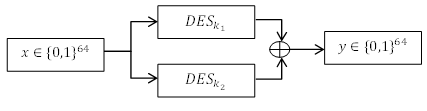
\includegraphics[width=0.5\linewidth]{scheme02}}
\end{figure} 
Маємо односторонню функцію.
\item 
Розглянем функцію $y=f(k,M)=E_{k}(M): \mathcal K \times \mathcal M \to \mathcal Y$. Якщо ШТ $Y$ більше
відстані єдиності, то по ШТ $Y$ можно знайти ключ $k$ і ВТ $M$. Але в загальному випадку, це можно зробити
лише овним перебором, а отже маємо односторонню функцію з секретом. 
\end{enumerate}
